\documentclass[border=5pt]{standalone}
\usepackage{tikz}
\usetikzlibrary{arrows}
\usetikzlibrary{shapes}
\usepackage{enumitem}
\usepackage{bm}
\usetikzlibrary{arrows,decorations.pathmorphing,backgrounds,fit,positioning,shapes.symbols,chains}
\usepackage[top=1in, bottom=1in, left=1in, right=1in]{geometry}
%\usepackage[active,tightpage]{preview}
%\title{}
%\author{}
%\date{}
\begin{document}

\pagenumbering{gobble}

%\begin{figure}[h!]

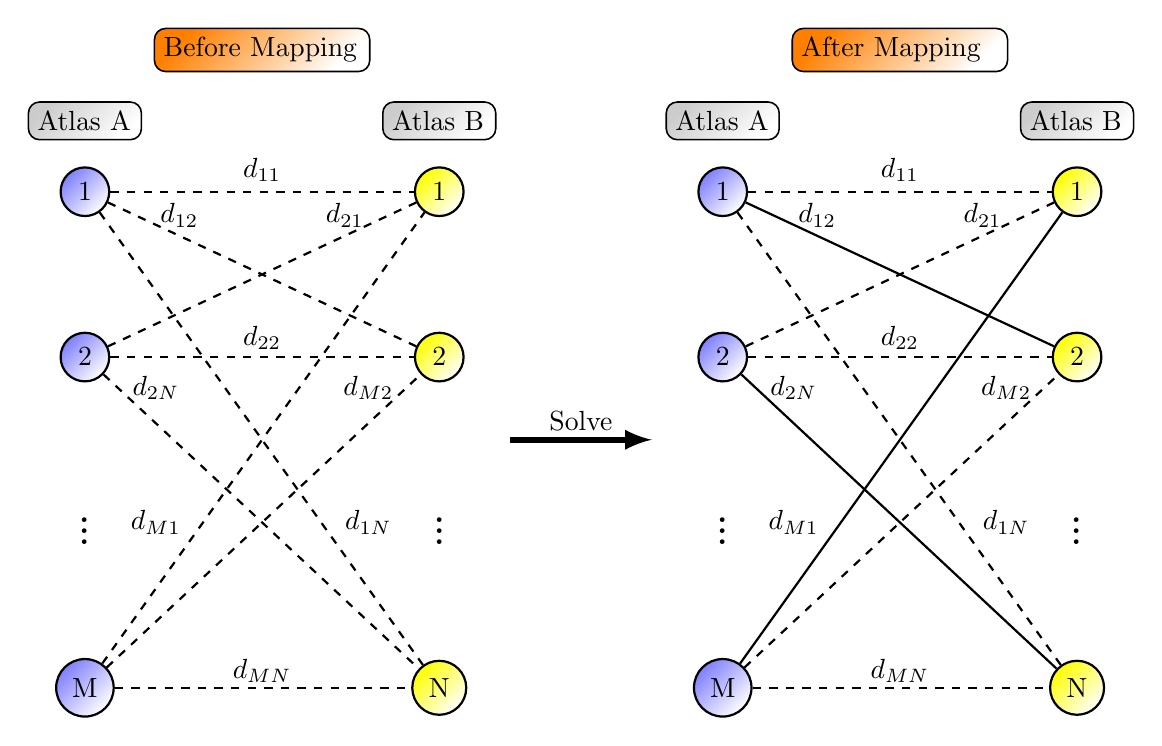
\begin{tikzpicture}[>=stealth, thick, scale=0.3]
						       \node[rectangle,draw=black,rounded corners,text width=2.5cm, line width=0.2mm,fill=orange,left color=orange, shading angle=45] at (7.5,6) (unmapped) {Before Mapping};
                               \node[rectangle,draw=black,rounded corners,text width=1.2cm,line width=0.2mm,fill=black!20, left color=black!20,shading angle=45] at (0,3) (title) {Atlas A};
                               \node[rectangle,draw=black,rounded corners,text width=1.2cm,line width=0.2mm,fill=black!20, left color=black!20,shading angle=45] at (15,3) (title) {Atlas B};
                               \node[circle, draw,fill=blue!50, left color=blue!50, shading angle=45] (A1) at (0,0) {1};
                               \node[circle, draw,fill=blue!50, left color=blue!50, shading angle=45] (A2) at (0,-7) {2};
                               \node[circle] (A3) at (0,-14) {\huge\vdots};
                               \node[circle, draw,fill=blue!50, left color=blue!50, shading angle=45] (A4) at (0,-21) {M};
                               \node[circle, draw,fill=yellow, left color=yellow, shading angle=45] (B1) at (15,0) {1};
                               \node[circle, draw,fill=yellow, left color=yellow, shading angle=45] (B2) at (15,-7) {2};
                               \node[circle] (B3) at (15,-14) {\huge\vdots};
                               \node[circle, draw,fill=yellow, left color=yellow, shading angle=45] (B4) at (15,-21) {N};
                               
                               \draw [thick,dashed] (A1) to node [above] {$d_{11}$} (B1);
							   \node[circle] (d12) at (4,-1) {$d_{12}$};
							   \draw [thick,dashed] (A1) to node [above] {} (B2);
							   \draw [thick,dashed] (A1) to node [above] {} (B4);
							   \node[circle] (d1N) at (12,-14) {$d_{1N}$};
							   \draw [thick,dashed] (A2) to node [above] {} (B1);
							   \node[circle] (d21) at (11,-1) {$d_{21}$};
							   \draw [thick,dashed] (A2) to node [above] {} (B2);
							   \node[circle] (d22) at (7.5,-6.2) {$d_{22}$}; 
							   \draw [thick,dashed] (A2) to node [above] {} (B4);
							   \node[circle] (d2N) at (3,-8.3) {$d_{2N}$};
							   \draw [thick,dashed] (A4) to node [above] {} (B1);
							   \node[circle] (dM1) at (3,-14) {$d_{M1}$};
							   \draw [thick,dashed] (A4) to node [above] {} (B2);
							   \node[circle] (dM2) at (12,-8.3) {$d_{M2}$};
							   \draw [thick,dashed] (A4) to node [above] {} (B4);
							   \node[circle] (dMN) at (7.5,-20.3) {$d_{MN}$};
                               
                               \node[rectangle,text width=2cm] at (23,-9.7) {Solve};
                               \draw [-latex,line width=0.8mm] (18,-10.5) -- (24,-10.5);
                               
                               \node[rectangle,draw=black,rounded corners,text width=2.5cm, line width=0.2mm,fill=orange,left color=orange, shading angle=45] at (34.5,6) (unmapped) {After Mapping};
                               \node[rectangle,draw=black,rounded corners,text width=1.2cm,line width=0.2mm,fill=black!20, left color=black!20,shading angle=45] at (27,3) (title) {Atlas A};
                               \node[rectangle,draw=black,rounded corners,text width=1.2cm,line width=0.2mm,fill=black!20, left color=black!20,shading angle=45] at (42,3) (title) {Atlas B};
                               \node[circle, draw,fill=blue!50, left color=blue!50, shading angle=45] (mA1) at (27,0) {1};
                               \node[circle, draw,fill=blue!50, left color=blue!50, shading angle=45] (mA2) at (27,-7) {2};
                               \node[circle] (mA3) at (27,-14) {\huge\vdots};
                               \node[circle, draw,fill=blue!50, left color=blue!50, shading angle=45] (mA4) at (27,-21) {M};
                               \node[circle, draw,fill=yellow, left color=yellow, shading angle=45] (mB1) at (42,0) {1};
                               \node[circle, draw,fill=yellow, left color=yellow, shading angle=45] (mB2) at (42,-7) {2};
                               \node[circle] (mB3) at (42,-14) {\huge\vdots};
                               \node[circle, draw,fill=yellow, left color=yellow, shading angle=45] (mB4) at (42,-21) {N};
                               
                               \draw [thick,dashed] (mA1) to node [above] {$d_{11}$} (mB1);
                               \node[circle] (d12) at (31,-1) {$d_{12}$};
                               \draw [thick] (mA1) to node [above] {} (mB2);
                               \draw [thick,dashed] (mA1) to node [above] {} (mB4);
                               \node[circle] (d1N) at (39,-14) {$d_{1N}$};
                               \draw [thick,dashed] (mA2) to node [above] {} (mB1);
                               \node[circle] (d21) at (38,-1) {$d_{21}$};
                               \draw [thick,dashed] (mA2) to node [above] {} (mB2);
                               \node[circle] (d22) at (34.5,-6.2) {$d_{22}$}; 
                               \draw [thick] (mA2) to node [above] {} (mB4);
                               \node[circle] (d2N) at (30,-8.3) {$d_{2N}$};
                               \draw [thick] (mA4) to node [above] {} (mB1);
                               \node[circle] (dM1) at (30,-14) {$d_{M1}$};
                               \draw [thick,dashed] (mA4) to node [above] {} (mB2);
                               \node[circle] (dM2) at (39,-8.3) {$d_{M2}$};
                               \draw [thick,dashed] (mA4) to node [above] {} (mB4);
                               \node[circle] (dMN) at (34.5,-20.3) {$d_{MN}$};
                               
                               
                               %\node[circle, draw] (i) at (50,-4) {$i$};
                               %\node[circle, draw] (j) at (50,-12) {$j$};
                               
                               %\draw [arrows={-angle 90}] (i) to node [right] {$u_{ij}$} (j);

\end{tikzpicture}

%\end{figure}

\end{document}